\documentclass[12pt, letterpaper, twoside]{article}
\usepackage[utf8]{inputenc}
\usepackage{titling}
\usepackage{amsmath}
\usepackage{mathtools}
\usepackage{cmsrb}
\usepackage[OT2,T1]{fontenc}
\usepackage[serbian]{babel}
\usepackage{amsmath}
\usepackage{tikz}
\usetikzlibrary{shapes,shadows,arrows}
\tikzstyle{line} = [draw, -stealth, thick]
\usepackage{graphicx}
\DeclareUnicodeCharacter{2212}{-}
\usepackage[export]{adjustbox}
\graphicspath{ {./images/} }
\makeatletter
\newcommand{\mathleft}{\@fleqntrue\@mathmargin0pt}
\newcommand{\mathcenter}{\@fleqnfalse}
\makeatother
\title{ % 
    Ensemble - Boosting Methods
    \\ }

\author{Emilija Mirković, Sanja Živanović}
\date{December 2022.}
\begin{document}
\maketitle
\begin{center}
\textbf{\large{ 1.1 Boosting Methods}} 

\end{center}
\hspace*{4ex} Ensemble methods are techniques that increase model precision (accuracy of results, predictions) by combining several different models in order to create one that is highly reliable.
There are several types of ensemble methods, and in this paper we will describe one of the most significant: \textbf{Boosting methods}.\\
\hspace*{4ex} Boosting belongs to the group of \textbf{Sequential Ensemble Techniques} that generate base learners in a sequence that promotes dependence between them. In this way, the performance of the model is further improved by increasing weights to learners that were previously misclassified. Boosting was originally designed to be used for classification problems, but it can also be used for regression problems.\\
\hspace*{4ex}Basically, model boosting is done by training the model by improving on the shortcomings of earlier versions of it. The idea behind the creation of this method was to create a procedure that would combine the results of multiple "weak" \space classifiers to create one powerful set of all that makes the least error of all (committee).
\begin{center}
\textbf{\large{1.1 \emph{AdaBoost}}} 
\end{center}
\hspace*{4ex}\emph{AdaBoost} (short for \emph{Adaptive Boosting}) is one of the most popular and widely used boosting algorithms.
The founders of this method, Yoav Freund and Robert Shapire (year 1995.) who originally named it \emph{"AdaBoost.M1."}, solved the difficulties of earlier boosting algorithms with this invention. 
\\\hspace*{4ex} Suppose we have a training set $\{x_i,y_i\}$ and each $x_i$ has a paired $y_i$ representing the output variable encoded with $y_i \in \{-1,1\}$. Also, a weak classifier $G(x)$ is given which makes a prediction and takes one of the values from the set $G(x_j)\in\{-1,1\}$ for each $x_j$. The idea is that for each round of training there is a new, improved classifier, so we will develop a set of weak classifiers over time $\{G_1,...G_T\}$.
\\\hspace*{4ex}Initially, all weights are set equally and in each round of training, the weights of the misclassified elements are increased, and more focus is invested in the more difficult (weighted) elements.
On the training set, the error is calculated as follows:\begin{equation}
\bar{err}=\frac{1}{N}\sum_{i=1}^{N}I(y_i\neq G(x_i))
\end{equation}
while the expected error rate on the following predictions is:\\
$E_{XY}I(Y\neq G(X))$.
\\
\\
\\\hspace*{4ex}In the scheme below we will describe the algorithm \emph{AdaBoost.M1}. In each round of training, weights are assigned to certain elements of the set, which is why we later call it a "weighted set".
Labels $G_1(x),...,G_M(x)$ denote classifiers for a certain training stage (each stage of training has its own improved classifier) trained on these sets.
\\
\\
\\
\begin{tikzpicture}[scale=2]
\tikzstyle{ann} = [draw=none,fill=none,right]
\matrix[nodes={draw, ultra thick, fill=blue!20},
        row sep=0.3cm,column sep=0.5cm] {
\node[draw,fill=red!30,ellipse,text width=2cm](1) 
  {training set $G_1(x)$}; &
\node[draw,fill=cyan!30,ellipse,text width=2cm](2)
  {weighted set $G_2(x)$}; &
\node[draw,fill=cyan!30,ellipse,text width=2cm](3)
  {weighted set $G_3(x)$}; &
\node[draw,fill=cyan!30,ellipse,text width=2cm](4)
  {weighted set $G_M(x)$};\\
};
\path [line] (1) -- (2);
\path [line] (2) -- (3);
\path [line] (3) -- (4);
\end{tikzpicture}
\\
\\
Here, we will introduce the coefficients $\alpha_i$ that indicate the contribution of the corresponding $G_i(x)$ in the sense that they give more influence to a more accurate classifier. Formula for the last (best) classifier obtained by the previously described procedure is:
\begin{equation*}
G(x)=sign [\sum_{m=1}^{M}\alpha_m G_m(x)]
\end{equation*}
\\
\textbf{The final prediction} is made by improving and combining the classifiers during this process. 
\\
At this point, we will introduce the term \textbf{weight}, mark them with $w_1, w_2,...,w_N$ and assume that they are initially set to: $w_i=1/N$. 
During this process, we apply them to each element of the training set $(x_i,y_i), i=1,2,...N$ and this is how the data is modified step by step.
\begin{center}
\large{\emph{1.1.1 Method}}
\end{center}
I) the classifier is trained on the data in the usual way\\
II) the classification algorithm is applied to weighted observations\\
III) previous applies to iterations $m=2,3,...M$\\
M) classifier performance $G_{m-1}(x)$: correctly classified observations have a reduced weight, while incorrectly classified ones have an increased weight 
\\ Observations that are difficult to classify correctly have a greater impact and as the procedure continues (the iterations alternate), the difference between them becomes more and more obvious. Therefore, new, time-improved classifiers will focus more on elements of the training set that were misclassified by their predecessors.
\begin{center}
\large{\emph{1.1.2 AdaBoost.M1.} algorithm}\\
\end{center}
Now we will describe the mathematical part of the functioning of the AdaBoost algorithm.\\\\
1. set initial weights $w_i=\frac{1}{N},i=1,...N$.\\\\
2. for values m=1,...,M:\\
\hspace*{4ex}(a)\space using the current weight $w_i$ adjust the classifier $G_m(x)$ on the training set; that current classifier is induced on difficult observations\\\\
\hspace*{4ex}(b)\space calculate the resulting weighted error rate:
\begin{equation*}
err_m=\frac{\sum_{i=1}^N w_i I(y_i\neq G_m(x_i))}{\sum_{i=1}^N w_i}
\end{equation*}\\
\hspace*{4ex}(c)\space determine the coefficients: $\alpha_m=\log(\frac{1-err_m}{err_m})$\\\\
\hspace*{4ex}(d)\space set: $w_i=w_i*\exp [\alpha_m I(y_i\neq G_m(x_i))], i=1,2,...N.$. Here, the individual weights of each observation are updated for the next iteration\\\\
3. calculating the final prediction: $G(x)=sign[\sum_{m=1}^M\alpha_m G_m(x)]$\\\\\\
The factor $\exp(\alpha_m)$ scales the weights of observations misclassified by $G_m(x)$.
In this way, such observations increase the influence for inducing the next classifier $G_{m+1}(x)$. \\
A weak classifier is one whose predictive power is little better than random guessing. The quality of this algorithm is that it greatly improves the weak classifier, i.e. reduces its error.
The figure below illustrates how the classifier's error rate decreases as the boosting iterations unfold.\\\\
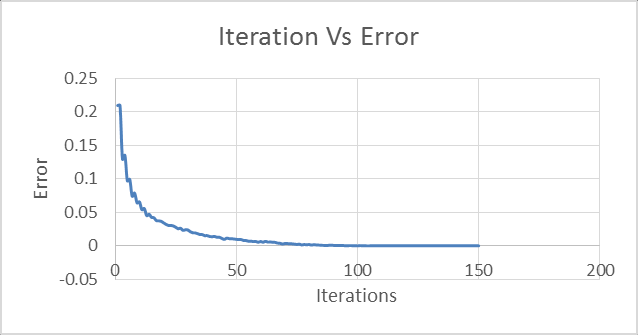
\includegraphics[width=13cm, height=7cm]{2}\\
\begin{center}
\textbf{\large{\\1.2 Boosting fits an Additive Model}\\}
\end{center}
Various classification and regression models can be represented as a linear combination of some simpler models. The formula for the generalized additive model is:
\begin{equation*}
f(x)=\sum_{m=1}^M \beta_m b_m(x;\gamma_m),
\end{equation*}
the variables in the previous model are:\\
- $x$ input data,\\
- $\{\beta_m,\gamma_m\}$ model parameters,\\
- $b_m(x;\gamma_m)$ are some arbitrary, simple functions with variable x\\\\
Amplification can be connected to additive models in that it represents a way of fitting additive expansion into a set of elementary functions (which in our case are the classifiers $G_m(x)\in\{-1,1\}$). In that case, the expansions of the elementary functions take the form of a generalized additive model.\\\\
How is the fitting of these models done?\\
-The model parameters $\{\beta_m,\gamma_m\}$ are estimated by minimizing a loss function (L, either quadratic or likelihood-based) that measures the prediction errors over the entire training set $\{x_n,y_n\}$:
\begin{equation*}
min_{\{\beta_m,\gamma_m\}_1^M} \sum_{i=1}^N L(y_i, \sum_{m=1}^M \beta_m b_m(x_i;\gamma_m)).
\end{equation*}
that is,
\begin{equation*}
\{\beta_m^*,\gamma_m^*\}_1^M=argmin_{\{\beta_m,\gamma_m\}_1^M}\sum_{i=1}^N L(y_i, \sum_{m=1}^M \beta_m b_m(x_i;\gamma_m)).
\end{equation*}
This calculation can be demanding, depending on the shape of the loss function and the basis functions $b_m(x;y)$.
\begin{center}
\textbf{\large{\\1.3 Forward Stagewise Additive Modeling}\\}
\end{center}
As already discussed, direct optimization of the loss function can be computationally challenging. However, if it is an alternative case where there is only one basic function, it can make our job a lot easier:
\begin{equation*}
min_{\beta,\gamma}\sum_{i=1}^N L(y_i,\beta b_m(x_i;\gamma)).
\end{equation*}
The idea behind forward stepwise modeling is to successively add new basis functions to approximate the solution of the original minimization problem:
\begin{equation*}
min_{\{\beta_m,\gamma_m\}_1^M} \sum_{i=1}^N L(y_i, \sum_{m=1}^M \beta_m b(x_i;\gamma_m)).
\end{equation*}
without changing the parameters that have been added.\\
The following algorithm will demonstrate the operation of forward stepwise modeling. It will be necessary to obtain a solution for the basis function $b(x;\gamma_m)$ and for the corresponding coefficient $\beta_m$ (in each iteration) which is then added to $f_{m-1}(x)$. In this way $f_m(x)$ is obtained and the process is repeated for the next iteration.\\
\begin{center}
\large{1.3.1 Forward Stagewise Modeling algorithm}\\
\end{center}
1. set $f_0(x)=0$.\\
2. for values of m from 1 to M:\\
\hspace*{6ex}(a)\space calculate:
\begin{equation*}
(\beta_m,\gamma_m)=argmin_{\beta,\gamma}\sum_{i=1}^N L(y_i,f_{m-1}(x_i)+\beta b(x_i;\gamma)).
\end{equation*}
\hspace*{6ex}(b)\space set $f_m(x)=f_{m-1}(x)+\beta_m b(x;\gamma_m)$\\\\
We will extract arguments of the loss function that we mentioned above $L(y_i,f_{m-1}(x_i)+\beta b(x_i;\gamma))$.\\
We distinguish between probability-based and squared-error loss functions. In the case of squared-error loss function, we set the well-known formula:
\begin{equation*}
L(y,f(x))=(y-f(x))^2,
\end{equation*}
and when the extracted arguments are inserted into this function we get:
\begin{equation*}
L(y_i,f_{m-1}(x_i)+\beta b(x_i;\gamma)) = (y_i-f_{m-1}(x_i)-\beta b(x_i;\gamma))^2,
\end{equation*}
Here, the most valuable addend is $\beta_mb(x;\gamma_m)$ which represents the residuals of this models residuals (or something close to residuals) and a
Ovde je najznačajniji sabirak $\beta_mb(x;\gamma_m)$ koji predstavlja reziduale ovog modela (ili nešto najbliže rezidualima) i dodaje se ekspanziji u svakoj iteraciji. Sa druge strane, prvi sabirak možemo obeležiti sa  $r_{im}=y_i-f_{m-1}(x_i)$ i on nam označava ostatak modela i-te observacije.\\\\
\begin{center}
\textbf{\large{\\1.4 Eksponential loss and boosting method \emph{AdaBoost} }\\}
\end{center}
How does the AdaBoost model fit into the whole story of the additive model and forward stagewise modeling?\\
-AdaBoost fits the additive model using stepwise modeling by:
\begin{itemize}
\item taking the binary classifier $G_m(x):R->\{-1,1\}$ for the elementary functions $b_m$
\item taking an exponential loss as the loss function
\end{itemize}
\begin{equation*}
L(y,f(x))=\exp(-y f(x))
\end{equation*}
Now that we know what the loss function looks like and what elementary functions are, we can solve the previously mentioned problems.
\begin{itemize}
\item We will start from a familiar expression
\begin{equation*}
(\beta_m,\gamma_m)=argmin_{\beta,\gamma}\sum_{i=1}^N L(y_i,f_{m-1}(x_i)+\beta b(x_i;\gamma)).
\end{equation*}
\item then insert known parameters
\begin{equation*}
(\beta_m,G_m)=argmin_{\beta,G}\sum_{i=1}^N \exp[-y_i(f_{m-1}(x_i)+\beta G(x_i))]
\end{equation*}
\item for the required weights configured in the expressions for the AdaBoost model (and applied to each observation), we will take $w_i=\exp(-y_i f_{m-1}(x_i))$
\item this is the correct form for the weight because it depends neither on the coefficient $\beta$ nor on the classifier $G(x)$
\begin{equation*}
(\beta_m,G_m)=argmin_{\beta,G}\sum_{i=1}^N w_i^{(m)} \exp(-\beta  y_i G(x_i)) (1.1)
\end{equation*}
\item the previous expression was derived in order to be able to add in each iteration the coefficient $\beta_m$ and the classifier $G_m$
\item In general, the weights in the AdaBoost model are different for each subsequent iteration. Considering that our chosen weights depend on the function $f_{m-1}(x_i)$, it can be concluded that the values of the weights themselves change as we go through the iterations (which was the initial idea)
\item now we need to split the data into two sets to decompose the sum above:
\item sada je potrebno da podelimo podatke u dva skupa da bismo razložili gornju sumu:
\begin{enumerate}
\item $I_1=\{y_i=G(x_i)\}$ 
\item $I_2=\{y_i\not=G(x_i)\}$
\end{enumerate}
\item dividing the sum into two
\begin{equation*}
(\beta_m,G_m)=argmin_{\beta,G}(e^{-\beta}\sum_{y_i=G(x_i)} w_i^{(m)} +e^{\beta}\sum_{y_i\not=G(x_i)}w_i^{(m)})
\end{equation*}
\begin{equation*}
(\beta_m,G_m)=argmin_{\beta,G}(e^{-\beta}\sum_{i=1}^N w_i^{(m)} +(e^{\beta}-e^{-\beta})\sum_{i=1}^N w_i^{(m)}I(y_i\not=G(x_i)))
\end{equation*}
\item in the previous equation, when we fix a value greater than zero of the coefficient $\beta_m$, we can obtain its solution and thus the expression of the optimal value for $G_m$
\end{itemize}
 \begin{equation*}
G_m=argmin_G\sum_{i=1}^N w_i^{(m)}I(y_i\neq G(x_i)) (1.2.)
\end{equation*}
This tells us that $G_m$ is actually a classifier that minimizes the weighted prediction error rate, given that the $w_i^{(m)}$ are weights assigned to the i-th element of the training set.\\
Now, naturally, we can also obtain the solution of equation 1.1 for the coefficient $\beta$.
\begin{itemize}
\item Let's go back to the expression
\begin{equation*}
(\beta_m,G_m)=argmin_{\beta,G}(e^{-\beta}\sum_{y_i=G(x_i)} w_i^{(m)} +e^{\beta}\sum_{y_i\not=G(x_i)}w_i^{(m)})
\end{equation*}
\item now we need to take the derivative with respect to the parameter $\beta$ and set it to zero in order to determine its minimum
\begin{equation*}
\frac{d(e^{-\beta}\sum_{y_i=G(x_i)} w_i^{(m)} +e^{\beta}\sum_{y_i\not=G(x_i)}w_i^{(m)})}{d\beta_m} = 0
\end{equation*}
\item the solution for $\beta$ is:
\end{itemize}
\begin{equation*}
\beta_m=\frac{1}{2}\log \frac{1-err_m}{err_m} (1.3)
\end{equation*}
where $err_m$ is the minimized weighted error rate
\begin{equation*}
err_m=\frac{\sum_{i=1}^N w_i^{(m)}I(y_i\neq G_m(x_i))}{\sum_{i=1}^N w_i^{(m)}}. (1.4)
\end{equation*}
Now it is necessary to examine the rule for updating weights, that is, how they change through iterations
\begin{equation*}
 \begin{aligned}
w_i^{(m+1)} &=exp(-y_if_m(x_i))\\
& =exp(-y_i(f_{m-1}(x_i)+\beta_mG_m(x_i)))\\
& =w_i^{(m)}exp(-\beta_m y_i G_m(x_i))\\
& =w_i^{(m)}exp(2\beta_mI(y_i\not=G_m(x_i)))exp(-\beta_m)
\end{aligned}
\end{equation*}
Now we go back to the \emph{AdaBoost} algorithm once we have gone through all its elements (we know where they come from):
\begin{enumerate}
\item we set the value for the weights $w_i=\frac{1}{N},i=1,...,N$
\item for m values from 1 to M:\\
\hspace*{4ex}(a) using the current weight $w_i$, adapt the classifier $G_m(x)$ on the training set\\
\hspace*{4ex}(b)\space determine the resulting weighted error rate:
\begin{equation*}
err_m=\frac{\sum_{i=1}^N w_i I(y_i\neq G_m(x_i))}{\sum_{i=1}^N w_i}
\end{equation*}\\
\hspace*{4ex}(c)\space determine the coefficients: $\alpha_m=\log(\frac{1-err_m}{err_m})$\\\\
\hspace*{4ex}(d)\space update the weights so that the following expression holds:\\ \hspace*{6ex}$w_i=w_i*\exp [\alpha_m I(y_i\neq G_m(x_i))], i=1,2,...N.$.
\item calculating the final prediction (algorithm output): $G(x)=sign[\sum_{m=1}^M\alpha_m G_m(x)]$
\end{enumerate}
It can be noted that we have taken $\alpha_m=2\beta_m$ for ease of notation.\\ 
From all of the above, we conclude that \emph{AdaBoost.M1} minimizes the exponential loss criterion $L(y,f(x))=\exp(-yf(x))$ using additive forward modeling.\\
\begin{center}
\textbf{\large{1.5 Other loss functions and Motivation for choosing Exponential Loss }\\}
\end{center}
By using exponential loss we can almost always get a simple AdaBoost algorithm and that is the main reason we choose it.\\
We will now examine what exactly it is assessing.
[Fridman paper, year 2000.] It can be shown that:
\begin{equation*}
f^*(x)=argmin_{f(x)}E_{Y|x}(e^{-Yf(x)})=\frac{1}{2}\log\frac{P(Y=1|x)}{P(Y=-1|x)},
\end{equation*}
from here we can get the probability that Y is correctly classified, i.e. that it is valid:
\begin{equation*}
P(Y=1|x)=\frac{1}{1+e^{-2f^*(x)}}.
\end{equation*}
The AdaBoost algorithm gives us half the logarithmic chance that Y will take the value 1. Furthermore, this justifies the use of its sign for the final classifier
\begin{equation*}
G_M(x) -> G(x)=sign [\sum_{m=1}^{M}\alpha_m G_m(x)].
\end{equation*}
The choice of the loss function is closely related to the complexity of the calculation and the robustness of the algorithm itself.The following loss functions can be used for classification:
\begin{itemize}
\item \textbf{0/1 loss}: $I\{sign(f(x))\not=y\}$
\item \textbf{binomial deviation}: $log(1+exp(-2yf))$
\item \textbf{loss of soft margin}: $(1-yf)I\{yf>1\}$ (SVM algoritham is used for this case)
\item \textbf{exponential loss} $exp(-yf(x))$ (AdaBoost algorithm is used in this case)
\end{itemize}
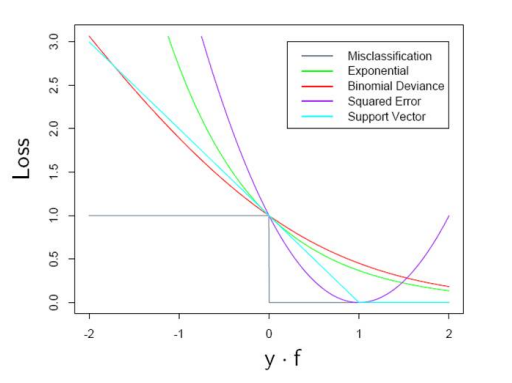
\includegraphics[width=11cm, height=7cm]{3}
\\\\"Loss" present a misclassification.\\
The following loss functions can be used for regression:\begin{itemize}
\item \textbf{squared error loss}: $(y-f(x))^2$
\item \textbf{an absolute loss}: $|y-f(x)|$
\item \textbf{Huber's loss}: $L(y,f)=$
\begin{enumerate}
\item \hspace*{10ex} $(y-f(x))^2$, ako je $|y-f(x)|<\delta$
\item \hspace*{10ex}$\delta(|y-f(x)|-\frac{\delta}{2})$, otherwise
\end{enumerate}
\end{itemize}  
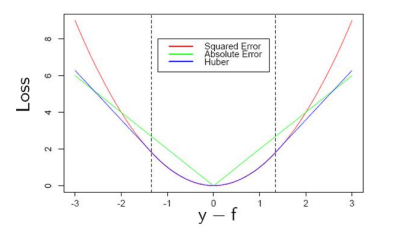
\includegraphics[width=11cm, height=7cm]{4}

\end{document}





